\documentclass[compress]{beamer}
\usepackage{ifthen}

\title{Status Report on Track-based Alignment}
\author{Jim Pivarski}
\institute{Texas A\&M University}
\date{ 9 February, 2007}

\setbeamertemplate{navigation symbols}{}
\setbeamertemplate{headline}{\includegraphics[height=1 cm]{../cmslogo} \hspace{0.1 cm} \includegraphics[height=1 cm]{../tamulogo} \hfill
\begin{minipage}{9 cm}
\vspace{-0.75 cm} \small
\begin{center}
\ifthenelse{\equal{\insertpagenumber}{1}}{}{\insertsection}
\end{center}
\end{minipage} \hfill
\begin{minipage}{1 cm}
\vspace{-0.75 cm} \small
\begin{center}
\ifthenelse{\equal{\insertpagenumber}{1}}{}{\insertpagenumber/23}
\end{center}
\end{minipage}}

%% \xdefinecolor{verylightgray}{rgb}{0.95,0.95,0.95}
%% \beamertemplateshadingbackground{verylightgray}{white}
\xdefinecolor{dkred}{rgb}{0.7,0,0}
\xdefinecolor{dkblue}{rgb}{0,0,0.7}

\begin{document}
\frame{\titlepage}
\section*{Track-based Alignment --- Jim Pivarski}

\begin{frame}
  \frametitle{Overview}
  \begin{description}
    \item[Our goal:] to improve high-$p_T$ muon resolution at \mbox{14~TeV (primary)}
      and 0.9~TeV (secondary)
    \item[Deliverables:] muon alignment data stream, software,
    well-studied HIP procedure, and alignment constants
  \end{description}
  \begin{center}
    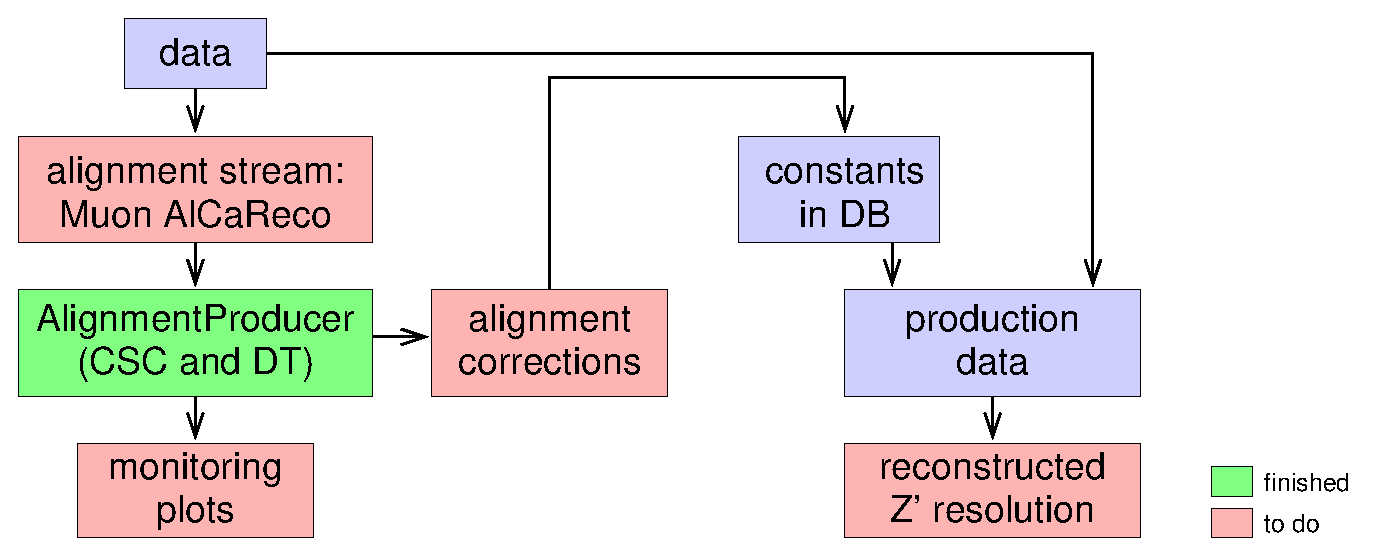
\includegraphics[width=\linewidth]{deliverables}
  \end{center}
\end{frame}

\section*{Track-based Alignment Stream --- Jim Pivarski}

\begin{frame}
  \frametitle{Alignment Stream}

  \vspace{-0.25 cm}
  \hspace{-0.5 cm}
  \begin{tabular}{p{0.81\linewidth} p{0.15\linewidth}}
    \hspace{0.1 cm}
    \begin{minipage}{\linewidth}
      \begin{itemize}
      \item Events of interest
	\begin{itemize}
          \item $W\to\mu\nu$ and $Z\to\mu\mu$ for 14~TeV
	  \item $b\to\mu X$, beam halo, and/or cosmics for 0.9~TeV
	  \item Just $Z\to\mu\mu$ for now
	\end{itemize}
      \end{itemize}
    \end{minipage} &
    \begin{minipage}{\linewidth}
      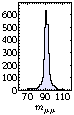
\includegraphics[width=\linewidth]{zpeak}
    \end{minipage}
  \end{tabular}

  \vspace{-0.3 cm}
  \begin{itemize}\setlength{\itemsep}{0.3 cm}
    \item<2-> Background studies
      \begin{itemize}
        \item Define cuts, optimize signal/rate
	\item $Z\to\mu\mu$ like sign minus opposite sign
      \end{itemize}

    \item<3-> Deweight muon chamber hits in alignment track fit
      \begin{itemize}
	\item Muon hits introduce a bias, though bias $\to$ 0 with iteration
	\item Need fewer muons: $N_{\mbox{\scriptsize muons}} \propto {\sigma_{\mbox{\scriptsize resid}}}^2$
	\item Weight $=$ 0 for now (tracker only)
      \end{itemize}

    \item<4-> AlCaReco format
      \begin{itemize}
	\item Currently includes only local muon reconstruction
	\item We need tracker fits and global muons!
      \end{itemize}

  \end{itemize}
\end{frame}

\section*{Track-based Alignment Software --- Jim Pivarski}

\begin{frame}
  \frametitle{Software: updated AlignmentProducer}

  \begin{itemize}
    \item Included muon chamber alignables and removed
      tracker-dependent assumptions
    \item Requred a reorganization of track refitter and
      Trajectory-calculating code \hfill \only<1>{\textcolor{dkblue}{CMS Week}}\only<2>{\textcolor{dkblue}{Now}}
  \end{itemize}

  \begin{center}
    \only<1>{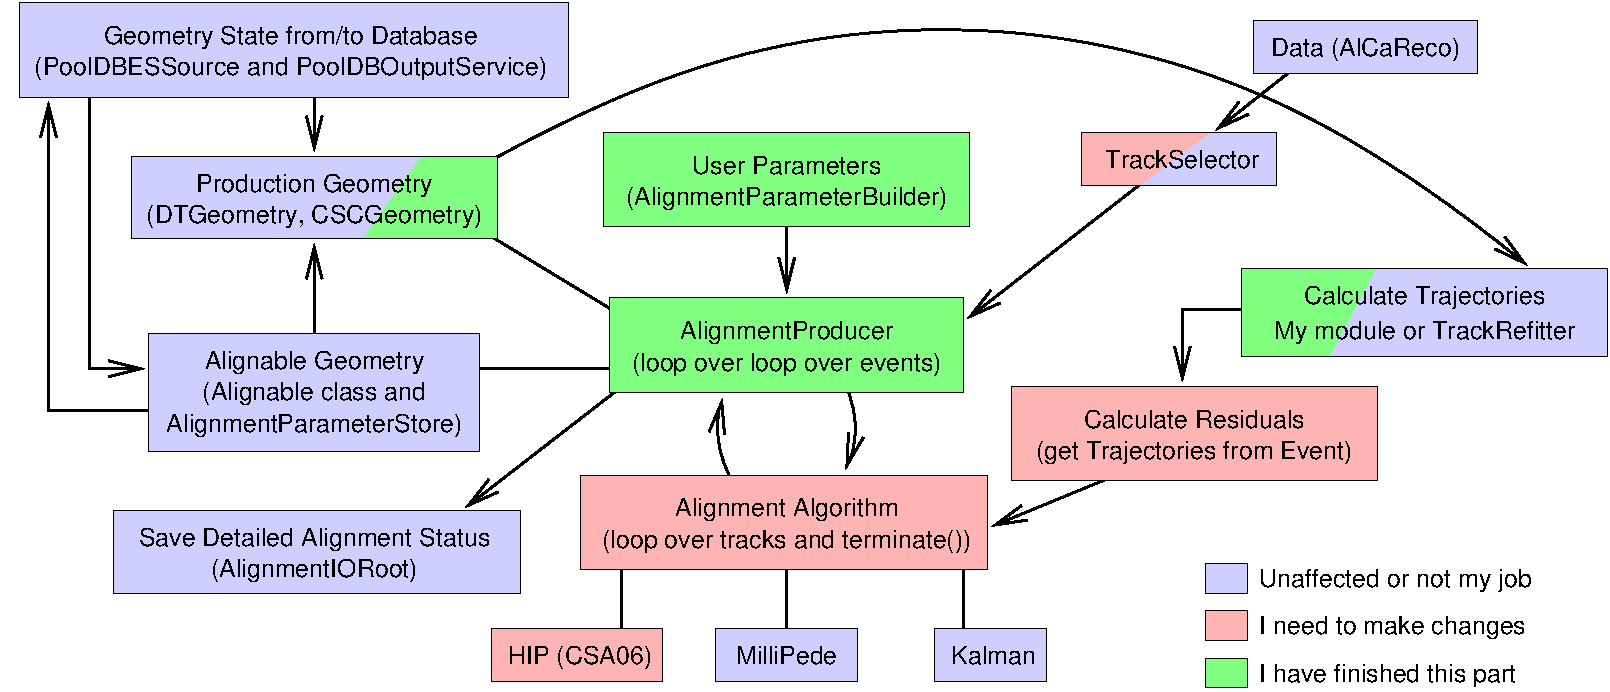
\includegraphics[height=4 cm]{flow_chart_old}}
    \only<2>{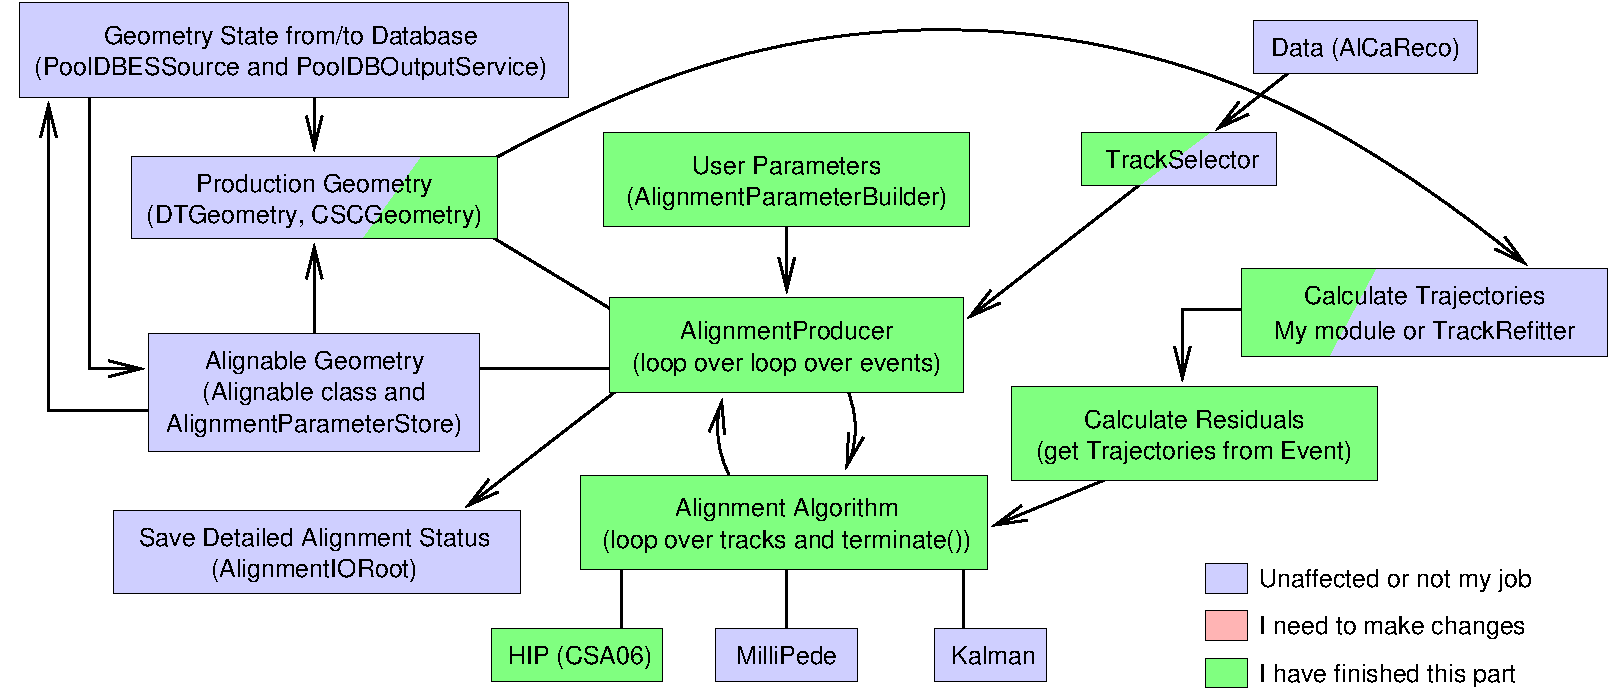
\includegraphics[height=4 cm]{flow_chart}}
  \end{center}

  \vspace{-0.25 cm}
  \begin{itemize}
    \item Updates are in CVS, but not all bug-fixes
  \end{itemize}
\end{frame}

\begin{frame}
  CommonAlignment framework can now\ldots

  \vspace{0.25 cm}
  \begin{tabular}{p{0.5\linewidth} p{0.45\linewidth}}
    \begin{minipage}{\linewidth}
      \begin{itemize}
	\item move muon geometry \\ (DT and CSC)
        \item calculate muon residuals.
      \end{itemize}
      Accessible to all 3 algos: \\
      \textcolor{dkblue}{HIP}, MillePede, and Kalman
    \end{minipage} &
    \begin{minipage}{\linewidth}
      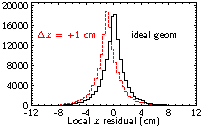
\includegraphics[width=\linewidth]{residual_hist}
    \end{minipage}
  \end{tabular}

  \vfill
  \uncover<2>{\begin{minipage}{\linewidth}

      \textcolor{dkblue}{HIP Algorithm:} move geometry to weighted mean of residuals (track
      minus hit), transformed to parameter space ($x$, $y$, $z$, $\phi_x$, $\phi_y$, $\phi_z$),

\vspace{0.1 cm}
\[ \begin{array}{c c}
  \mbox{alignment} \\
  \mbox{corrections} \end{array} =
\left(\begin{array}{c c}
  \mbox{ } \\
  \mbox{ } \end{array}\right)
\left(\begin{array}{c c}
  \mbox{weighted mean} \\
  \mbox{of residuals} \end{array}\right)
\left(\begin{array}{c c}
  \mbox{ } \\
  \mbox{ } \end{array}\right)^{-1}_,
\]

\vspace{0.15 cm}
      chamber-by-chamber.

  \end{minipage}}

\end{frame}

\begin{frame}
  \frametitle{Corrected treatment of 1-dimensional hits}

  Our first alignment moved DTs by tens of cm, but not CSCs\ldots
  \begin{itemize}
    \item CSA06 HIP assumed all sensors are 2D
    \item Axial DT hits have no $y$ information
  \end{itemize}

  \vspace{-0.5 cm}
  \begin{center}
    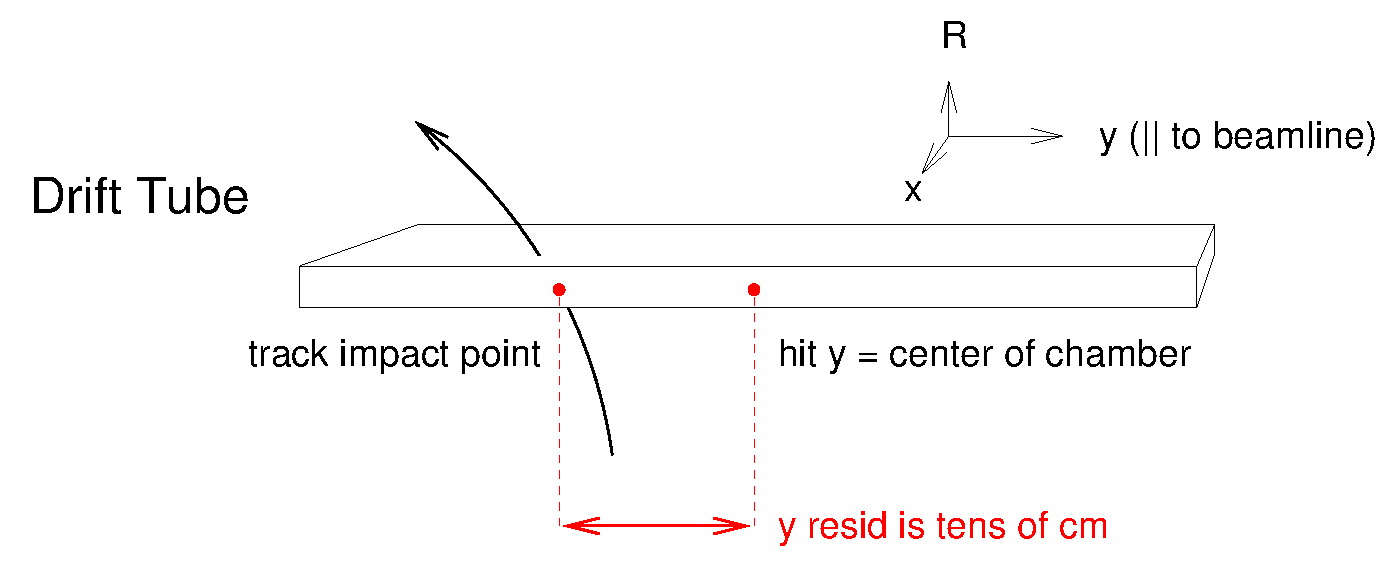
\includegraphics[width=0.9\linewidth]{onedimhit}
  \end{center}

  \vspace{-0.25 cm}
  \begin{itemize}
    \item We modified the algorithm such that these hits contribute to
    \mbox{$x$ alignment} but not $y$ alignment (we set $1/{\sigma_{r_y}}^2 = 0$)
  \end{itemize}
\end{frame}

\begin{frame}
  \frametitle{Demonstration of muon alignment!}

  Alignment output, starting from\ldots

  \begin{tabular}{p{0.45\linewidth} p{0.45\linewidth}}
    \begin{minipage}{\linewidth}
      \begin{center}
	an ideal alignment
      \end{center}
    \end{minipage} &
    \begin{minipage}{\linewidth}
      \begin{center}
	\only<1>{all chambers $\Delta x = +1$ cm}
	\only<2>{all $\Delta \phi_z = +10$ mrad}
      \end{center}
    \end{minipage} \\
    \begin{minipage}{\linewidth}
      \begin{center}
	\only<1>{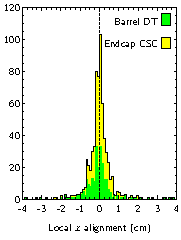
\includegraphics[width=\linewidth]{init_alignments_x}}
	\only<2>{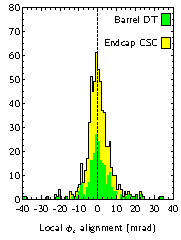
\includegraphics[width=\linewidth]{init_alignments_phiz}}
      \end{center}
    \end{minipage} &
    \begin{minipage}{\linewidth}
      \begin{center}
	\only<1>{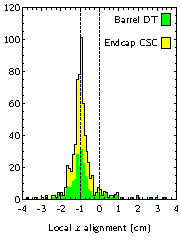
\includegraphics[width=\linewidth]{x_alignments_x}}
	\only<2>{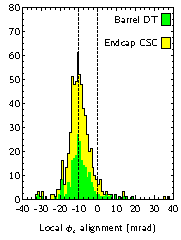
\includegraphics[width=\linewidth]{phiz_alignments_phiz}}
      \end{center}
    \end{minipage} 
  \end{tabular}
\end{frame}

\begin{frame}
  \frametitle{Alignment Uncertainties}
  
  \begin{itemize}
    \item Derive purely from residual uncertainties
    \item Too small to account for RMS of chamber corrections
  \end{itemize}

  \vspace{-0.25 cm}
  \begin{center}
    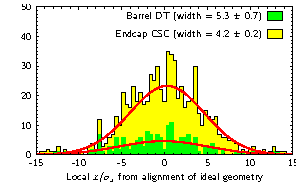
\includegraphics[width=0.9\linewidth]{alignoutput}
  \end{center}
\end{frame}

\section*{Track-based Alignment Monitoring --- Jim Pivarski}

\begin{frame}
  \frametitle{Monitoring Alignment for Quality Control}
  \begin{itemize}\setlength{\itemsep}{0.75 cm}
    \item Need to produce constants {\it and} confidence that they are correct, on a regular basis

    \item Include all helpful plots in the HIP alignment package

    \item Present the most useful for routine monitoring

    \item HIP can diagnose and validate MillePede and Kalman
  \end{itemize}
\end{frame}

\begin{frame}
  \frametitle{Monitoring: Trends in Residual Profiles}

  \vspace{-1 cm}
  \begin{center}

    \begin{tabular}{p{0.35\linewidth} p{0.35\linewidth} p{0.35\linewidth}}
      \begin{minipage}{\linewidth}
      \end{minipage} &
      \begin{minipage}{\linewidth}
	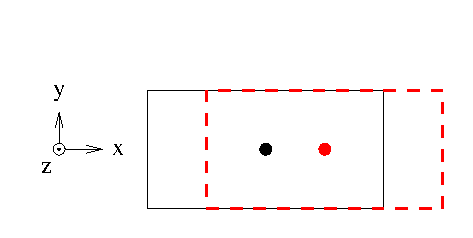
\includegraphics[width=0.8\linewidth]{dof_x}
      \end{minipage} &
      \begin{minipage}{\linewidth}
	\hspace{-0.8 cm}
	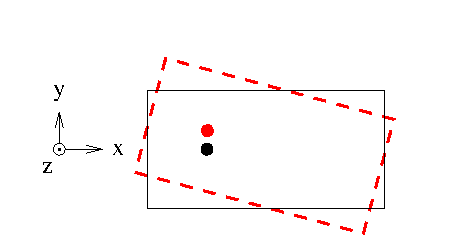
\includegraphics[width=0.8\linewidth]{dof_phiz}
      \end{minipage} \\
      \begin{minipage}{\linewidth}
      \end{minipage} &
      \begin{minipage}{\linewidth}
	\hspace{0.4 cm}
	\small $x$: offset in $r_x$
      \end{minipage} &
      \begin{minipage}{\linewidth}
	\hspace{-0.6 cm}
	\small $\phi_z$: $r_x$ linear in $y$
      \end{minipage} \\
      & & \\
      \begin{minipage}{\linewidth}
	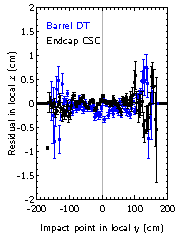
\includegraphics[width=\linewidth]{init_xresid_vs_y}
      \end{minipage} &
      \begin{minipage}{\linewidth}
	\hspace{-0.7 cm}
	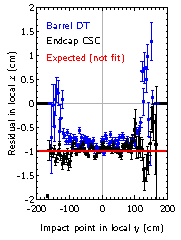
\includegraphics[width=\linewidth]{x_xresid_vs_y}
      \end{minipage} &
      \begin{minipage}{\linewidth}
	\hspace{-1.4 cm}
	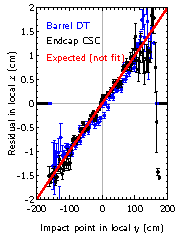
\includegraphics[width=\linewidth]{phiz_xresid_vs_y}
      \end{minipage}
    \end{tabular}
  \end{center}
\end{frame}

\begin{frame}
  \frametitle{Monitoring: Convergence}
  \begin{itemize}
    \item Corrections should get smaller with every iteration
  \end{itemize}

  \vspace{-0.5 cm}
  \begin{center}
    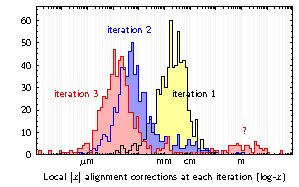
\includegraphics[width=0.85\linewidth]{three_iterations_really}
  \end{center}

  \vspace{-0.5 cm}
  \begin{itemize}
    \item Unknown problem with some chambers in iteration 3\ldots
  \end{itemize}
\end{frame}

\begin{frame}
  \frametitle{Monitoring: Coverage}
  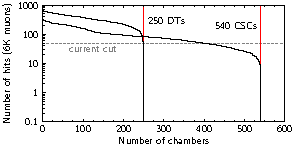
\includegraphics[width=\linewidth]{coverage}

  \begin{itemize}
    \item Keep track of which chambers see no/too few hits
    \item Versus $\eta$ and $\phi$
  \end{itemize}
\end{frame}

\section*{Track-based Alignment Data Needed --- Jim Pivarski}

\begin{frame}
  \frametitle{$W$ and $Z$ data needed at 14~TeV}
  \begin{itemize}
    \item First projection using a complete alignment simulation!
  \end{itemize}

  \vspace{-0.5 cm}
  \begin{center}
    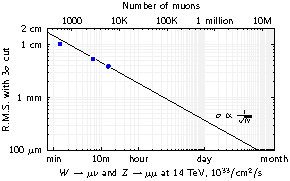
\includegraphics[width=0.85\linewidth]{time_projection}
  \end{center}

  \vspace{-0.5 cm}
  \begin{itemize}
    \item Conservative: muon chambers excluded from track-fit
  \end{itemize}
\end{frame}

\section*{Track-based Alignment Conclusions --- Jim Pivarski}

\begin{frame}
  \frametitle{Schedule (copied from CMS Week talk)}

  \renewcommand{\arraystretch}{1.5}
  \begin{tabular}{p{0.18\linewidth} p{0.75\linewidth}}
    Deadline & Task \\ \hline

    \textcolor{dkblue}{1 Jan,} \hfill \textcolor{dkblue}{2007} & \textcolor{dkblue}{Finish integrating muon chambers into alignment framework} \\

      1 Mar, \hfill 2008 & Transition CSA06Alignment to HIPAlignment and
      develop low-level diagnostics suite \\

      1 Apr & \textcolor{dkblue}{Prototype} and study realistic alignment procedure, assuming a
      source of muons \\
 
      1 May & Evaluate possible sources ($W\to\mu\nu$, $Z\to\mu\mu$,
      cosmics, or good muon) and finalize routine \\

      1 Jun & Document everything
  \end{tabular}
\end{frame}

\begin{frame}
  \frametitle{Relationship with hardware alignment}
  \begin{itemize}
    \item<1-> Limitations of track-based alignment for 2007 data (0.9~TeV,
      low lumi) are still unknown

    \item<2-> Hardware alignment is sensitive to shorter time intervals
      \begin{center}
	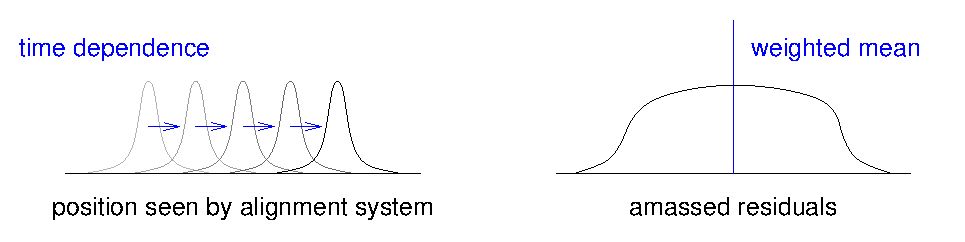
\includegraphics[width=0.85\linewidth]{time_peaks}
      \end{center}

       \mbox{\hspace{-0.3 cm}} Alignment system can resolve edges \\ \mbox{\hspace{-0.3 cm}} of natural alignment datasets

      \vspace{0.3 cm}
    \item<3-> Error ellipses are not collinear
    \item<3-> Different systematic uncertainties
  \end{itemize}

  \hfill \begin{minipage}{0.4\linewidth} \vspace{-2.8 cm} \uncover<3->{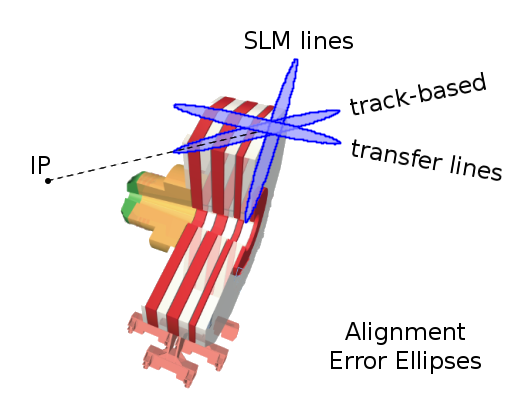
\includegraphics[width=\linewidth]{error_ellipses}} \end{minipage}
\end{frame}

\end{document}
